\section{Feedforward Networks}
\emph{Deep feedforward networks}, also called \emph{feedforward neural networks} or \emph{multilayer perceptrons} (MLPs) are basic deep learning models.
Their main purpose is to approximate some kind of function \(f^*(x)\).
Take for example a classification function \(y = f^*(x)\), where every input \(x\) maps to a class \(y\).
A feedforward network now aims to learn the best parameters \(\Theta\) for a function \(y = f(x, \Theta)\) that approximates \(f^*(x)\).

These models are \emph{networks} due to the fact that they can be represented by \emph{directed graphs}.
They are called \emph{feedforward networks} because the input \(x\) flows through these functions without any \emph{feedback} connections.
This means that the graph is \emph{acyclic}.
If the graph is \emph{not acyclic} and therefore \(feedback\) connections exist, we speak of \emph{recurrent neural networks}.

For example let \(f(x) = (f^3 \circ f^2 \circ f^1)(x) = f^3(f^2(f^1(x)))\).
We now define the \emph{depth} of a \emph{feedforward network} \(f\) as the number of functions that compose it.
Our example has a \emph{depth} of \(3\).
These kind of chains are very typical in \emph{neural networks}, as each function in the chain represents a layer in the \emph{directed acyclic graph}.
The last element of the chain (in our example \(f^1\)) and therefore the last layer in the graph is called the \emph{output layer} as it maps the input \(x\) to its final value.
If we think of \(f\) as a classifier function the elements of the \emph{codomain} of \(f^1\) are the classes.
Likewise, the elements of the \emph{domain} of the first function in the chain (in our example \(f^3\)) are the inputs of the network.
The first layer is called \emph{input layer}.
Layers between the \emph{input} and \emph{output} layer are called \emph{hidden layers}.

\subsection{Feedforward network graphs}
As proposed earlier we can also think of \emph{neural networks} as \emph{acyclic directed graphs}.
Loosely inspired by neuroscience, \emph{neurons} are interpreted as \emph{nodes} and \emph{synapses} as \emph{edges}.
Each \emph{node} now receives input from an arbitrary amount of neurons in the previous layer and computes an output with its own activation function.
An \emph{edges} on the other hand has a scalar \emph{weight}.
These \emph{weights} are now what can be adjusted to change the output of the neural network.

It is shown in  \cite{Nair-Hinton}, \cite{inproceedings}, that in most feedforward networks a \emph{rectifier linear units} (reLU) (\(f(x) = \text{max}(0, x)\)) activation function works best.
However, in certain cases other activation functions might perform better.
Such would be for example the \emph{swish} activation function (\(f(x) = x * \text{sigmoid}(x)\)), that tends to perform better than reLU on deeper models. \cite{DBLP:journals/corr/abs-1710-05941}

% Small sample neural network graph
\begin{figure}[h]
    \centering
    \label{fig:dnn-example}
    
    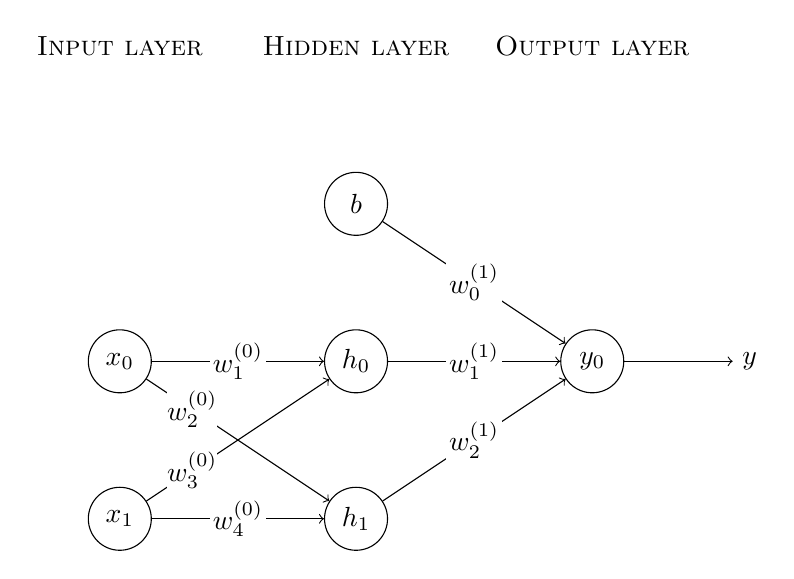
\begin{tikzpicture}
        \def\vert{2}
        \def\hori{3}
        \tikzstyle{place}=[circle, draw=black, minimum size=8mm]
        \tikzstyle{label}=[inner sep=1pt, fill=white]
        
        % Input
        \draw node at (0 * \hori, 4 * \vert) [black, ] {\textsc{Input layer}};
        
        \draw node at (0 * \hori, 2 * \vert) [place] (input_0) {$x_0$};	
        \draw node at (0 * \hori, 1 * \vert) [place] (input_1) {$x_1$};
        
        
        % Hidden
        \draw node at (1 * \hori, 4 * \vert) [black, ] {\textsc{Hidden layer}};
        
        \draw node at (1 * \hori, 3 * \vert) [place] (hidden_0) {$b$};
        \draw node at (1 * \hori, 2 * \vert) [place] (hidden_1) {$h_0$};	
        \draw node at (1 * \hori, 1 * \vert) [place] (hidden_2) {$h_1$};	
        
        % Output
        \draw node at (2 * \hori, 4 * \vert) [black, ] {\textsc{Output layer}};
        
        \draw node at (2 * \hori, 2 * \vert) [place] (output_0) {$y_0$};
        
        % Out
        \node at (8, 2 * \vert) [black, ] (out_0) {$y$};
		
        % Input -> Hidden
        % \foreach \i in {0,...,1}
        %  	 \foreach \j in {1,...,2}
        %		 \draw [->] (input_\i) to node[near start, below] {$w_{\i}^{(0)}$} (hidden_\j);
        \draw [->] (input_0) to node[label] {$w_{1}^{(0)}$} (hidden_1);
        \draw [->] (input_0) to node[label, near start, inner sep=0pt] {$w_{2}^{(0)}$} (hidden_2);
        \draw [->] (input_1) to node[label, near start, inner sep=0pt] {$w_{3}^{(0)}$} (hidden_1);
        \draw [->] (input_1) to node[label] {$w_{4}^{(0)}$} (hidden_2);
        
        
        % Hidden -> Output
        \foreach \i in {0,...,2}
		\foreach \j in {0,...,0}
        \draw [->] (hidden_\i) to node[label] {$w_{\i}^{(1)}$} (output_\j);
        
        \foreach \i in {0,...,0}
		\draw [->] (output_\i) to (out_\i);
        
    \end{tikzpicture}
    \caption{Example DNN with a single hidden layer}
\end{figure}

This DNN \fref{fig:dnn-example} can now also be described by its \emph{weight matrices}. 

We can represent the weights of the edges between two layers as a \emph{weight matrices} \(\fat{W} \in \mathbb{R}^{m \times n}\).
The input can be represented as a vector \({x \in \mathbb{R}^n}\).
Calculating the output of a neural network can therefore be achieved by iterative \emph{matrix-vector multiplication} and component-wise usage of the activation function on each layer.

For \fref{fig:dnn-example} the weight matrices are
\begin{equation}
    \fat{W}^{(0)} =
    \begin{pmatrix}
        w_{2}^{(0)} & w_{4}^{(0)} \\
        w_{3}^{(0)} & w_{5}^{(0)}
    \end{pmatrix}, \quad
    \fat{W}^{(1)} = 
    \begin{pmatrix}
        w_{1}^{(1)} & w_{2}^{(1)}
    \end{pmatrix}.
\end{equation}
With the corresponding bias vectors
\begin{equation}
    b^{(0)} =
    \begin{pmatrix}
        w_{0}^{(0)} \\
        w_{1}^{(0)}
    \end{pmatrix}, \quad
    b^{(1)} =
    \begin{pmatrix}
        w_{0}^{(1)}
    \end{pmatrix}.
\end{equation}
In order to get more \enquote{flexible} we add a \emph{bias} node to each layer.
This bias node always has an input of \(1\) and describes the constant in a linear equation.

Let \(f(x)\) now be the activation function and
\begin{equation}
    x =
    \begin{pmatrix}
        x_0 \\
        x_1
    \end{pmatrix},
\end{equation}
the input vector.
The output vector for \fref{fig:dnn-example} can be calculated by evaluating the following equations.
\begin{equation}
    x_0 =
    f(W^{(0)}x + b^{0}) =
    f(
    \begin{pmatrix}
        w_{2}^{(0)} & w_{4}^{(0)} \\
        w_{3}^{(0)} & w_{5}^{(0)}
    \end{pmatrix}
    \begin{pmatrix}
        x_0 \\
        x_1å
    \end{pmatrix}
    +
    \begin{pmatrix}
        w_{0}^{(0)} \\
        w_{1}^{(0)}
    \end{pmatrix}
    )
\end{equation}
\begin{equation}
    y =
    f(W^{(1)}x_0 + b^{1}) =
    f(
    \begin{pmatrix}
        w_{1}^{(1)} & w_{2}^{(1)}
    \end{pmatrix}
    x_0
    +
    \begin{pmatrix}
        w_{0}^{(1)}
    \end{pmatrix}
    )
\end{equation}
Where the activation function \(f\) is used component-wise.